\clearpage

\section{STARTUP}\label{sec:startup}\index{STURTUP}\index{self training}

\begin{notebox}
\textbf{Paper: } \fullcite{phoo_self-training_2021}
\vspace{5pt}

\href{https://openreview.net/forum?id=O3Y56aqpChA}{reviews}
\hspace{1cm}
\href{https://github.com/cpphoo/STARTUP}{code}
\hspace{1cm}
\href{run:/home/magda/Dropbox/Zot/Phoo_Hariharan_2021_Self-training for Few-shot Transfer Across Extreme Task Differences}{Local pdf}
\vspace{3pt}

Presented at CAIRO readings\index{CAIRO readings} 16/2/2022
\hfill Notes taken: 15/2/2022 \index{February 2022}
\end{notebox}

\begin{notebox}[colback=red!5]
\tldr 
\end{notebox}

\begin{notebox}[colback=yellow!5]
\textbf{Notes:} 
\begin{itemize}[nosep]
\item 
\end{itemize}
\end{notebox}

Few-shot learning\index{few-shot learning} when the source domain is very different from the target domain. Solution is in self-training in the target representation using an unlabelled dataset form the target domain.

Current sota few-shot methods are often outperformed by simple transfer with finetunning in cross-domain setups \cite{wallace_extending_2020,guo_broader_2020}.
The story is about the features extracted from the target domain follow some grouping logic derived from the base domain. This may not make much sense in the target domain as the classes may be completely different but induces a notion of similarity which is broader then the instance-based similarity of simCLR\parencite{chen_simple_2020} and similar. 

\begin{figure}[ht]
\centering
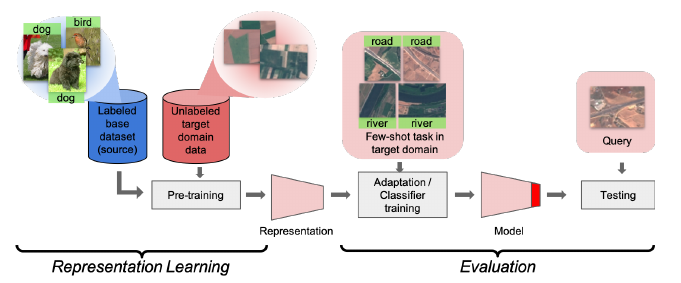
\includegraphics[width=10cm]{startup_Figure1.png}
\caption{bla}
\end{figure}
They have large labelled base dataset $D_B$, small (few-shot) labelled dataset from different domain $D_N$ and an unlabelled dataset from the same domain $D_u$(slightly bigger).
Operates in two phases
\begin{itemize}[nosep]
\item learn representations using $D_B$ and $D_u$
\item learn novel classes in few-shot setup from $D_N$
\end{itemize}
